\begin{columns}
  \begin{column}{0.35\textwidth}
    \centering

    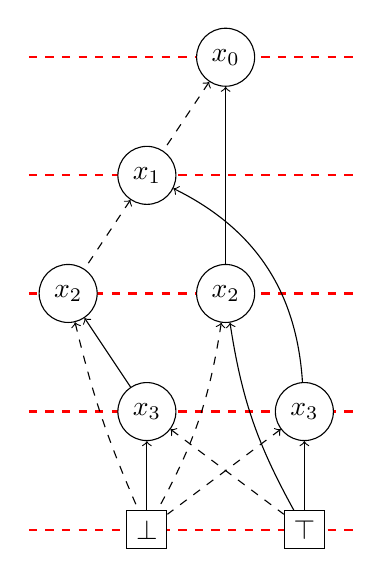
\begin{tikzpicture}
      % sweepline
      \onslide<2>     { \draw[red, thick, dashed] (-2.5,-6)   -- ++(4.2, 0); }
      \onslide<3>     { \draw[red, thick, dashed] (-2.5,-4.5) -- ++(4.2, 0); }
      \onslide<4>     { \draw[red, thick, dashed] (-2.5,-3)   -- ++(4.2, 0); }
      \onslide<5-13>  { \draw[red, thick, dashed] (-2.5,-1.5) -- ++(4.2, 0); }
      \onslide<14-22> { \draw[red, thick, dashed] (-2.5, 0) -- ++(4.2, 0); }

      % nodes
      \node[shape=circle, draw=black, fill=white] at ( 0, 0)
      (0) {$x_0$};

      \node[shape=circle, draw=black, fill=white] at (-1,-1.5)
      (1) {$x_1$};

      \node[shape=circle, draw=black, fill=white] at (-2,-3)
      (21) {$x_2$};
      \node[shape=circle, draw=black, fill=white] at ( 0,-3)
      (22) {$x_2$};

      \node[shape=circle, draw=black, fill=white] at (-1,-4.5)
      (31) {$x_3$};
      \node[shape=circle, draw=black, fill=white] at ( 1,-4.5)
      (32) {$x_3$};

      % leafs
      \node[shape=rectangle, draw=black, fill=white] at (-1,-6)
      (bot) {$\bot$};
      \node[shape=rectangle, draw=black, fill=white] at ( 1,-6)
      (top) {$\top$};

      % arcs
      \draw[<-, dashed]
        (0)  edge (1)
        (1)  edge (21)
        (21) edge[bend right=5] (bot)
        (22) edge[bend left=10] (bot)
        (31) edge (top)
        (32) edge (bot)
      ;

      \draw[<-]
        (0)  edge (22)
        (1)  edge[bend left] (32)
        (21) edge (31)
        (22) edge[bend right=10] (top)
        (31) edge (bot)
        (32) edge (top)
      ;
    \end{tikzpicture}
  \end{column}
  \begin{column}{0.35\textwidth}
    \centering

    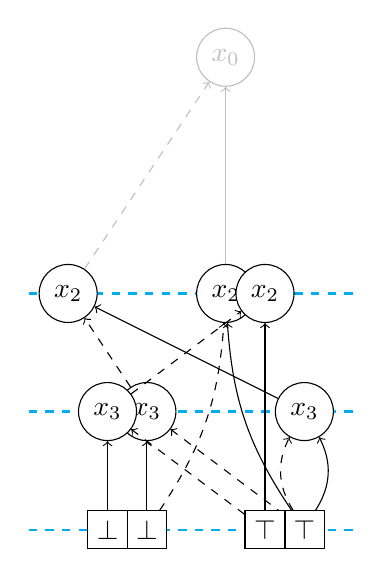
\begin{tikzpicture}
      % sweepline
      \onslide<7,13,16,22>
      { \draw[cyan, thick, dashed] (-2.5,-3)   -- ++(4.2, 0); }
      \onslide<8,12,17,21>
      { \draw[cyan, thick, dashed] (-2.5,-4.5) -- ++(4.2, 0); }
      \onslide<9,11,18,20>
      { \draw[cyan, thick, dashed] (-2.5,-6)   -- ++(4.2, 0); }

      % ----------------------------------------------------------------------
      % 1st Iteration (Apply)

      \onslide<7-14> {
        \node[shape=circle, draw=lightgray, fill=white] at ( 0, 0)
        (0) {\color{lightgray} $x_0$};

        \node[shape=circle, draw=black, fill=white] at (-2,-3)
        (21) {$x_2$};
        \node[shape=circle, draw=black, fill=white] at ( 0,-3)
        (22) {$x_2$};

        \draw[->, dashed, lightgray] (21) edge (0);
        \draw[->, lightgray] (22) edge (0);
      }

      \onslide<8-14> {
        \node[shape=circle, draw=black, fill=white] at (-1,-4.5)
        (31) {$x_3$};
        \node[shape=circle, draw=black, fill=white] at ( 1,-4.5)
        (32) {$x_3$};

        \draw[->, dashed]
          (31) edge (21)
        ;
        \draw[->]
          (32) edge (21)
        ;
      }

      \onslide<9-14> {
        \node[shape=rectangle, draw=black, fill=white] at (-1,-6)
        (bot) {$\bot$};
        \node[shape=rectangle, draw=black, fill=white] at ( 1,-6)
        (top) {$\top$};

        \draw[->, dashed]
          (bot) edge[bend right=15] (22)
          (top) edge (31)
          (top) edge[bend left] (32)
        ;
        \draw[->]
          (bot) edge (31)
          (top) edge[bend left=15] (22)
          (top) edge[bend right] (32)
        ;
      }

      % ----------------------------------------------------------------------
      % 2nd Iteration (Apply)

      \onslide<16-22> {
        \node[shape=circle, draw=black, fill=white] at ( 0.5,-3)
        (2) {$x_2$};
      }

      \onslide<17-22> {
        \node[shape=circle, draw=black, fill=white] at (-1.5,-4.5)
        (3) {$x_3$};

        \draw[->, dashed] (3) edge (2);
      }

      \onslide<18-22> {
        \node[shape=rectangle, draw=black, fill=white] at (-1.5,-6)
        (bot) {$\bot$};
        \node[shape=rectangle, draw=black, fill=white] at ( 0.5,-6)
        (top) {$\top$};

        \draw[->, dashed]
          (top) edge (3)
        ;
        \draw[->]
          (bot) edge (3)
          (top) edge (2)
        ;
      }
    \end{tikzpicture}
  \end{column}
  \begin{column}{2em}
    \centering
    \only<1-5,10-14,19->{$\implies$}%
    \only<6-9,15-18>{$\impliedby$}%
  \end{column}
  \begin{column}{0.35\textwidth}
    \centering

    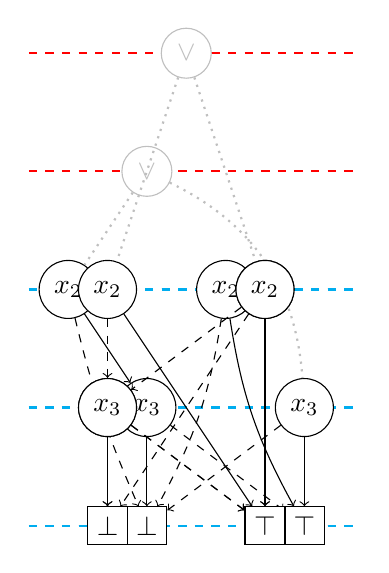
\begin{tikzpicture}
      % sweepline
      \onslide<2>     { \draw[red, thick, dashed] (-2.5,-6)   -- ++(4.2, 0); }
      \onslide<3>     { \draw[red, thick, dashed] (-2.5,-4.5) -- ++(4.2, 0); }
      \onslide<4>     { \draw[red, thick, dashed] (-2.5,-3)   -- ++(4.2, 0); }
      \onslide<5-13>  { \draw[red, thick, dashed] (-2.5,-1.5) -- ++(4.2, 0); }
      \onslide<14-22> { \draw[red, thick, dashed] (-2.5, 0) -- ++(4.2, 0); }

      \onslide<7,13,16,22>
      { \draw[cyan, thick, dashed] (-2.5,-3)   -- ++(4.2, 0); }
      \onslide<8,12,17,21>
      { \draw[cyan, thick, dashed] (-2.5,-4.5) -- ++(4.2, 0); }
      \onslide<9,11,18,20>
      { \draw[cyan, thick, dashed] (-2.5,-6)   -- ++(4.2, 0); }

      % ----------------------------------------------------------------------
      % 1st Iteration (Outer Reduce)

      \onslide <2-9> {
        \node[shape=rectangle, draw=black, fill=white] at (-1,-6)
        (bot) {$\bot$};
        \node[shape=rectangle, draw=black, fill=white] at ( 1,-6)
        (top) {$\top$};
      }

      \onslide <3-9> {
        \node[shape=circle, draw=black, fill=white] at (-1,-4.5)
        (31) {$x_3$};
        \node[shape=circle, draw=black, fill=white] at ( 1,-4.5)
        (32) {$x_3$};

        \draw[->, dashed]
          (32) edge (bot)
          (31) edge (top)
        ;
        \draw[->]
          (32) edge (top)
          (31) edge (bot)
        ;
      }

      \onslide <4-9> {
        \node[shape=circle, draw=black, fill=white] at (-2,-3)
        (21) {$x_2$};
        \node[shape=circle, draw=black, fill=white] at ( 0,-3)
        (22) {$x_2$};

        \draw[->, dashed]
          (22) edge[bend left=10] (bot)
          (21) edge[bend right=5] (bot)
        ;
        \draw[->]
          (22) edge[bend right=10] (top)
          (21) edge (31)
        ;
      }

      \onslide <5-9> {
        \node[shape=circle, draw=lightgray, fill=white] at (-1,-1.5)
        (1) {\color{lightgray} $\lor$};

        \draw[-, dotted, thick, lightgray]
          (1)  edge (21)
          (1)  edge[bend left] (32)
        ;
      }

      % ----------------------------------------------------------------------
      % 2nd Iteration (Inner + Outer Reduce)

      \onslide<11-18> {
        \node[shape=rectangle, draw=black, fill=white] at (-1.5,-6)
        (bot) {$\bot$};
        \node[shape=rectangle, draw=black, fill=white] at ( 0.5,-6)
        (top) {$\top$};
      }

      \onslide<12-18> {
        \node[shape=circle, draw=black, fill=white] at (-1.5,-4.5)
        (3) {$x_3$};

        \draw[->, dashed]
          (3) edge (top)
        ;
        \draw[->]
          (3) edge (bot)
        ;
      }

      \onslide<13-18> {
        \node[shape=circle, draw=black, fill=white] at (-1.5,-3)
        (21) {$x_2$};
        \node[shape=circle, draw=black, fill=white] at ( 0.5,-3)
        (22) {$x_2$};

        \draw[->, dashed]
          (22) edge (bot)
          (21) edge (3)
        ;
        \draw[->]
          (22) edge (top)
          (21) edge (top)
        ;
      }

      \onslide<14-18> {
        \node[shape=circle, draw=lightgray, fill=white] at (-0.5, 0)
        (0) {\color{lightgray} $\lor$};

        \draw[-, dotted, thick, lightgray]
          (0) edge (21)
          (0) edge (22)
        ;
      }

      % ----------------------------------------------------------------------
      % 3rd Iteration (Inner + Outer Reduce)

      \onslide<20-> {
        \node[shape=rectangle, draw=black, fill=white] at (-1.5,-6)
        (bot) {$\bot$};
        \node[shape=rectangle, draw=black, fill=white] at ( 0.5,-6)
        (top) {$\top$};
      }

      \onslide<21-> {
        \node[shape=circle, draw=black, fill=white] at (-1.5,-4.5)
        (3) {$x_3$};

        \draw[->, dashed] (3) edge (top);
        \draw[->] (3) edge (bot);
      }

      \onslide<22-23> {
        \node[shape=circle, draw=black, fill=white] at ( 0.5,-3)
        (2) {$x_2$};

        \draw[->, dashed] (2) edge (3);
        \draw[->] (2) edge (top);
      }

    \end{tikzpicture}
  \end{column}
\end{columns}